\documentclass[12pt]{article}
\usepackage{color}
\usepackage{graphicx}
\usepackage{booktabs}
\usepackage{amsmath}
\usepackage[utf8]{inputenc}
%\usepackage[german]{babel}
\usepackage{multirow}
\usepackage{siunitx}
\usepackage{pbox}
%\usepackage{tabularx}
\usepackage{multirow}
\usepackage{float}
\usepackage{amssymb,amsmath}
\makeatletter
\def\maketag@@@#1{\hbox{\m@th\normalfont\normalsize#1}}
\makeatother
\setlength{\parindent}{0pt}

%\addtolength{\textwidth}{1in}
%\addtolength{\textheight}{1in}
%\addtolength{\evensidemargin}{0.5in}
%\addtolength{\oddsidemargin}{-0.5in}
%\addtolength{\topmargin}{-0.6in}
%\addtolength{\bottommargin}{0.4in}


\usepackage[top = 2.50cm, bottom = 2.50cm, left = 2.75cm, right = 2.50cm]{geometry}

\renewcommand{\floatpagefraction}{1.0}


\begin{document}
\title{PHY118/119 \\ {\bf Übungsstunde 3 und 4: Arbeit, Leistung, Energie}}
\author{Assistent: Simon Flury \\E-mail: simon.flury@uzh.ch\\\\ }
\maketitle

\section{Wichtig!!!}
Dieses Dokument ist kein offizielles Dokument, es ist weder von Prof.Kilminster noch vom Hauptassistenten abgesegnet, somit kann sich nicht darauf bezogen werden und es wird auch keine Haftung für Fehler übernommen. Es dient einzig und allein als Lernunterstützung von mir an euch und bezieht sich ausschliesslich auf meine Übungsstunde.
\section{Arbeit, Leistung, Energie}
In den letzten beiden Wochen, sowie in der kommenden Woche, beschäftigen wir uns mit dem Thema: Arbeit, Leistung, Energie.
\\
\\
Arbeit im physikalischen Sinne ist definiert als $W = F*s$ also Kraft mal Weg und trägt die Einheit Joule $J = kgm/s^2$.
\\
Definition:
\begin{equation}
dW = \vec{F} \cdot d\vec{r}
\end{equation}
dies ist die differentielle Definition, lasst euch davon nicht verwirren, es bedeutet lediglich, dass $\dfrac{dW}{dr} = F$ also die Ableitung der Arbeit, nach dem Weg oder falls wir Mittelwerte betrachten $\dfrac{\Delta W}{\Delta r} = F$ die Arbeit über eine bestimmte Wegdifferenz ist gleich der aufgewendeten Kraft.
\begin{equation}
W_{1\rightarrow 2} = \int_{1}^2 \,dW = \int_{1}^2 \vec{F} \cdot d\vec{r}
\end{equation}
Somit ist die Arbeit die verrichtet wird, wenn man einen Körper vom Punkt 1 zum Punkt 2 bewegt, gleich der aufgewendeten Kraft integriert über die Strecke. (Da es sich hier um Vektoren handelt ist dies kein mal sondern ein Skalarprodukt, ihr könnt die Vektorpfeile aber auch einfach weglassen und mal schreiben.)
\\
\\
Leistung ist definiert als Arbeit pro Zeit, sprich
\begin{equation}
P = \dfrac{dW}{dt} = \dfrac{\vec{F} \cdot d\vec{r}}{dt} = \vec{F} \cdot \dfrac{d\vec{r}}{dt}
\end{equation}
und trägt die Einheit Watt was J/s, also Joule pro Sekunde entspricht.
\\
\\
Betrachten wir die Definition der Arbeit, bemerken wir schenll, dass Führungskräfte, welche per def. immer senkrecht zum Weg stehen, keine Arbeit verrichten. $\vec{F} \cdot \vec{r} \rightarrow F \cdot r\cdot \cos(\phi)$ da Führungskraft senkrecht zum Weg ist $\phi = 90^\circ$ und somit $cos(\phi) = 0$
\\
\\
Kommen wir nun zu einem wichtigen Satz, dem Energiesatz der Mechanik:
\\ Herleitung:
$\dfrac{dp}{dt} = F \rightarrow v \cdot \dfrac{dp}{dt} = F \cdot v \rightarrow m\cdot v \cdot \dfrac{dv}{dt} = P$ mit $P$ ist die Leistung gemeint. Somit gilt:$\dfrac{1}{2}m\cdot\dfrac{dv^2}{dt} = \dfrac{dW}{dt}$
Wir definieren nun $T = \dfrac{1}{2}mv^2$ als kinetische Energie, daraus folgt
\begin{equation}
\dfrac{dT}{dt} = \dfrac{dW}{dt}
\end{equation}
dies bedeutet, dass die Zunahme der kinetischen Energie gleich der von den Kräften geleisteten Arbeit ist.
\begin{equation}
T_2 - T_1 = \int_1^2 dT = W_{1\rightarrow 2}
\end{equation}
dies ist der \textbf{Energiesatz der Mechanik}\\
\\
Beispiel: Bremsweg eines Zuges.\\
\begin{figure}[H]
  \centering{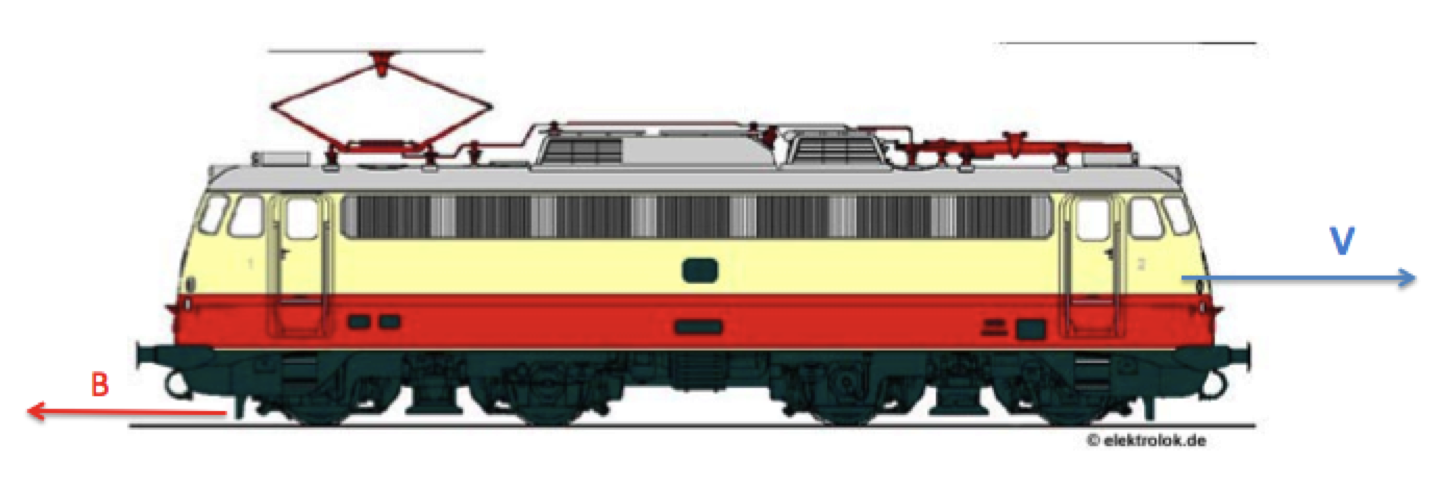
\includegraphics[width=0.4\textwidth]{Zug.png}}
  \caption{Zug mit Bremskraft B und Geschw. $v_1$}
  \label{fig:1teil}
\end{figure} 
Bremskraft $\vec{B}$\\
Anfang: $T_1 = \dfrac{m}{2}v_1^2$\\
Ende: $T_2 = \dfrac{m}{2}v_2^2 = 0$ da $v_2 = 0$\\
Arbeit: $W_{1\rightarrow 2} = \int_{1}^2 \vec{F} \cdot d\vec{r} = -\int_{1}^2 B \cdot dr = -B \int_{1}^2 dr = -B(r_2 - r_1)$ (das Minus kommt davon, dass B in die entgegengesetzte Richtung von v zeigt.\\
Nun gilt nach dem Energiesatz: $T_2 - T_1 = W_{1\rightarrow 2}$
somit $0-\dfrac{m}{2}v_1^2 = -B(r_2-r_1) \rightarrow r_2-r_1 = \dfrac{mv_1^2}{2B}$ dies ist der benötigte Bremsweg.

\subsection{Potentielle Enrgie von konservativen Kraftfeldern}
Es stellt sich nun natürlich die Frage, ob man $W$ in jedem Raumpunkt definieren kann?\\
Dazu muss gelten: $W$sprich das Integral über den Weg muss unabhängig vom gewählten Weg sein. Sprich \textcolor{blue}{ $W_{1\rightarrow 2} = \int \vec{F} \cdot d\vec{r}$} muss gleich \textcolor{red}{$W_{1\rightarrow 2} = \int \vec{F} \cdot d\vec{r}$} sein.
\begin{figure}[H]
  \centering{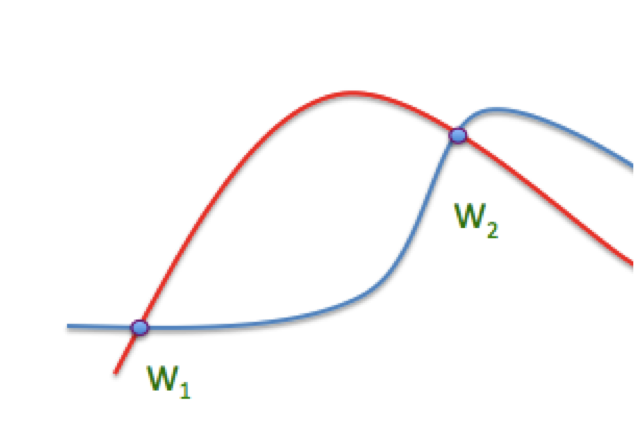
\includegraphics[width=0.4\textwidth]{Graphen.png}}
  \caption{Darstellung zweier möglicher Wege, mit Kreuzpunkten 1 und 2}
  \label{fig:1teil}
\end{figure}

Ist dies der Fall so spricht man von einer \textbf{konservativen Kraft}.
\\
\\
Die potentielle Energie einer konservativen Kraft wird nun wie folgt definiert:
\begin{equation}
V_2 - V_1 = -\int_{1}^2 \vec{F}\cdot d\vec{r}
\end{equation}
als das negative der geleisteten Arbeit oder in differentieller Schreibweise $dV = -\vec{F} \cdot d\vec{r}$.
Damit gilt nun $W_{1 \rightarrow 2} = T_2-T_1$ und $W_{1 \rightarrow 2} = -(V_2-V_1)$ woraus folgt $V_1+T_1 = V_2+T_2$ oder anders ausgedrückt
\begin{equation}
V+T = const
\end{equation}
Dies ist der \textbf{Energieerhaltungssatz der Mechanik für konservative Kräfte}. (Achtung: Reibungskraft zum Beispiel ist kein konservative Kraft!)
\\
Was passiert eigentlich wenn es sich um einen geschlossenen Weg handelt?
\begin{figure}[H]
  \centering{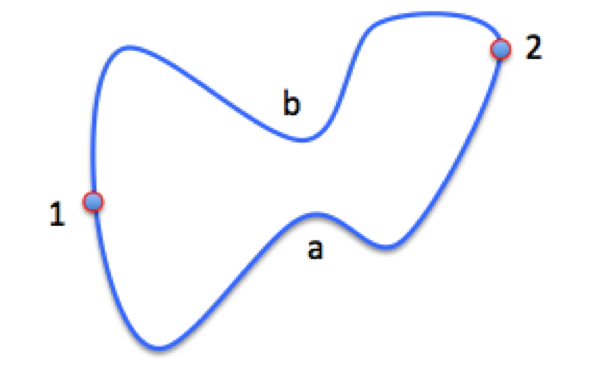
\includegraphics[width=0.4\textwidth]{geschWeg.png}}
  \caption{Darstellung eines geschlossenen Weges.}
  \label{fig:1teil}
\end{figure}
$W_{1 \rightarrow 2} = \int_{1b}^2 \vec{F} \cdot d\vec{s} + \int_{2a}^1 \vec{F} \cdot d\vec{s} = \int_{1b}^2 \vec{F} \cdot d\vec{s} - \int_{1a}^2 \vec{F} \cdot d\vec{s} = 0$ (=0 falls wegunabhängig)\\
\\ Kraftfeld ist konservativ $\Leftrightarrow W_{1 \rightarrow 1} = 0$ (geschlossener Weg)
\begin{equation}
\int_1^1 \vec{F} d\vec{s} = 0 \Leftrightarrow \oint \vec{F} \cdot d\vec{s}
\end{equation}
daher gilt: Kraftfeld ist konservativ $\Leftrightarrow \exists$ potentielle Energie $V$\\
(Falls ihr irritiert seit, wir schreiben immer $T \rightarrow E_{kin}$ und $V \rightarrow E_{pot}$)\\
\\
Für die Aufgaben, sowie allgemein für diese Vorlesung benötigt ihr jedoch lediglich diese Definitionen der verschiedenen Energien:
\begin{itemize}
$E_{pot} = mgh$ (Vorsicht, dass Nullniveau eures Systems könnt ihr selbst wählen, müsst jedoch konsistent bleiben.)
\end{itemize}
\begin{itemize}
$E_{kin} = \dfrac{1}{2}mv^2$
\end{itemize}
\begin{itemize}
$E_{Feder} = \dfrac{1}{2}Dx^2$ (Federenergie mit Federkonstanten $D$)
\end{itemize}

\section{Impulserhaltung}
Eine der wichtigsten physikalischen Eigenschaften eines Systems ist die Impulserhaltung, welche immer gilt. $p_i = p_f$ sprich der gesamte Impuls am Anfang ist gleich dem gesamten Impuls am Ende eines Vorgangs.\\
Gesamtimpuls: $\vec{p} = \sum m_i \cdot \vec{v_i}$\\
Die Änderung des Gesamtimpulses ist gleich der Summe der äusseren Kräfte:$\dfrac{d\vec{p}}{dt} = \sum \vec{F}_{aussen}$
\\
Ein gutes Beispiel für Impulserhaltung sind jegliche Stossprozesse:
\begin{itemize}
\textbf{elastische Stösse}: Körper bleiben unverändert, es gilt Energie und Impulserhaltung.
\end{itemize}
\begin{itemize}
\textbf{inelastische Stösse}: Körper verformen sich, mechanische Energie ist nicht erhalten, der Impuls jedoch schon.
\end{itemize}
\\
\\
Bei einen Zusammenstoss zweier Körper kommt es zu einer Impulsübetragung durch einen Kraftstoss.\\
Kraftstoss:
\begin{equation}
\vec{F(t)} = \dfrac{d\vec{p}}{dt} \rightarrow \vec{p_f}-\vec{p_i} = \int_i^f \vec{F} \cdot dt$
\end{equation}

\section{Aufgabe 1, Serie 4}
\begin{figure}[H]
  \centering{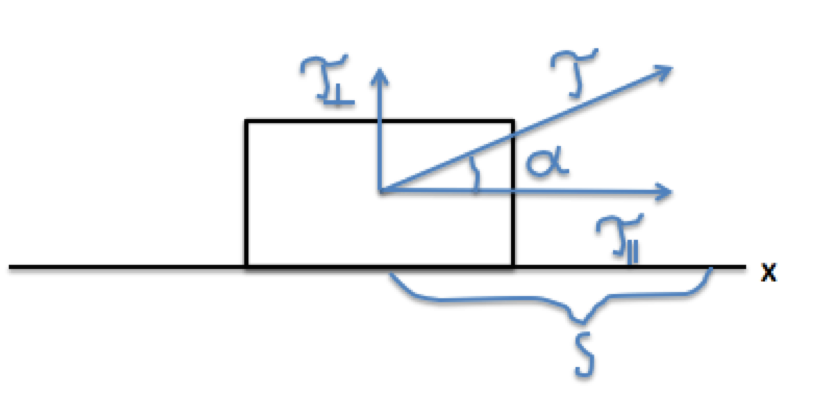
\includegraphics[width=0.4\textwidth]{Kiste.png}}
  \caption{Situation in der Aufgabe.}
  \label{fig:1teil}
\end{figure}
Nun ist in Teil a nach der Arbeit gefragt welche die Kraft$\tau$ verrichtet, sowie der Reibungsarbeit. Die Arbeit erhalten wir ganz einfach aus Kraft mal Weg und wenn ihr euch die Definition in Erinnerung ruft seht ihr sofort, dass wegem dem Konsinus des Skalarproduktes nur der zur x-Achse parallele Anteil der Kraft, Arbeit verrichtet. Somit gilt:
\begin{equation}
W_{\tau} = \tau \cdot s \cdot \cos(\alpha})
\end{equation}
Um nun noch die Reibungsarbeit zu berechen müssen wir erst die Normalkraft herausfinden, da $F_R = \mu_d F_N$\\
Der Körper erfährt keine resultierende Beschleunigung in y-Richtung, somit muss gelten: Summe der vertikalen Kräfte = 0.
\begin{equation}
F_N + \tau \cdot \sin(\alpha}) = mg \rightarrow F_N = mg-\tau \sin(\alpha)$
\end{equation}
daraus folgt direkt:
\begin{equation}
F_R = \mu_d \cdot (mg - \tau \sin(\alpha))$
\end{equation}
Die Arbeit erhalten wir nun wieder wie üblich aus Kraft mal Weg.
\begin{equation}
W_R = F_R \cdot s = \mu_d \cdot s \cdot (mg - \tau \cdot sin(\alpha))
\end{equation}

\end{document}
